\section{System Overview}
\label{overview}
Heimdall has two components. The first component is an app that is installed on a user's mobile device. The second component is a webservice that receives install, uninstall and update notifications when said activity occurs on the phone for any app. Upon intimation the server processes the list of heuristics that apply to the app at the moment and generates a set of actions for a system administrator. At this point the system administrator can take an appropriate action based on the detected threat level. At present we are working with the content provider heuristic to determine the impact of this vulnerability. The only solution that is possible, at the moment, is to uninstall the app and that notification is then sent back to the user's device automatically.

\begin{figure}[tb]
	\centering
	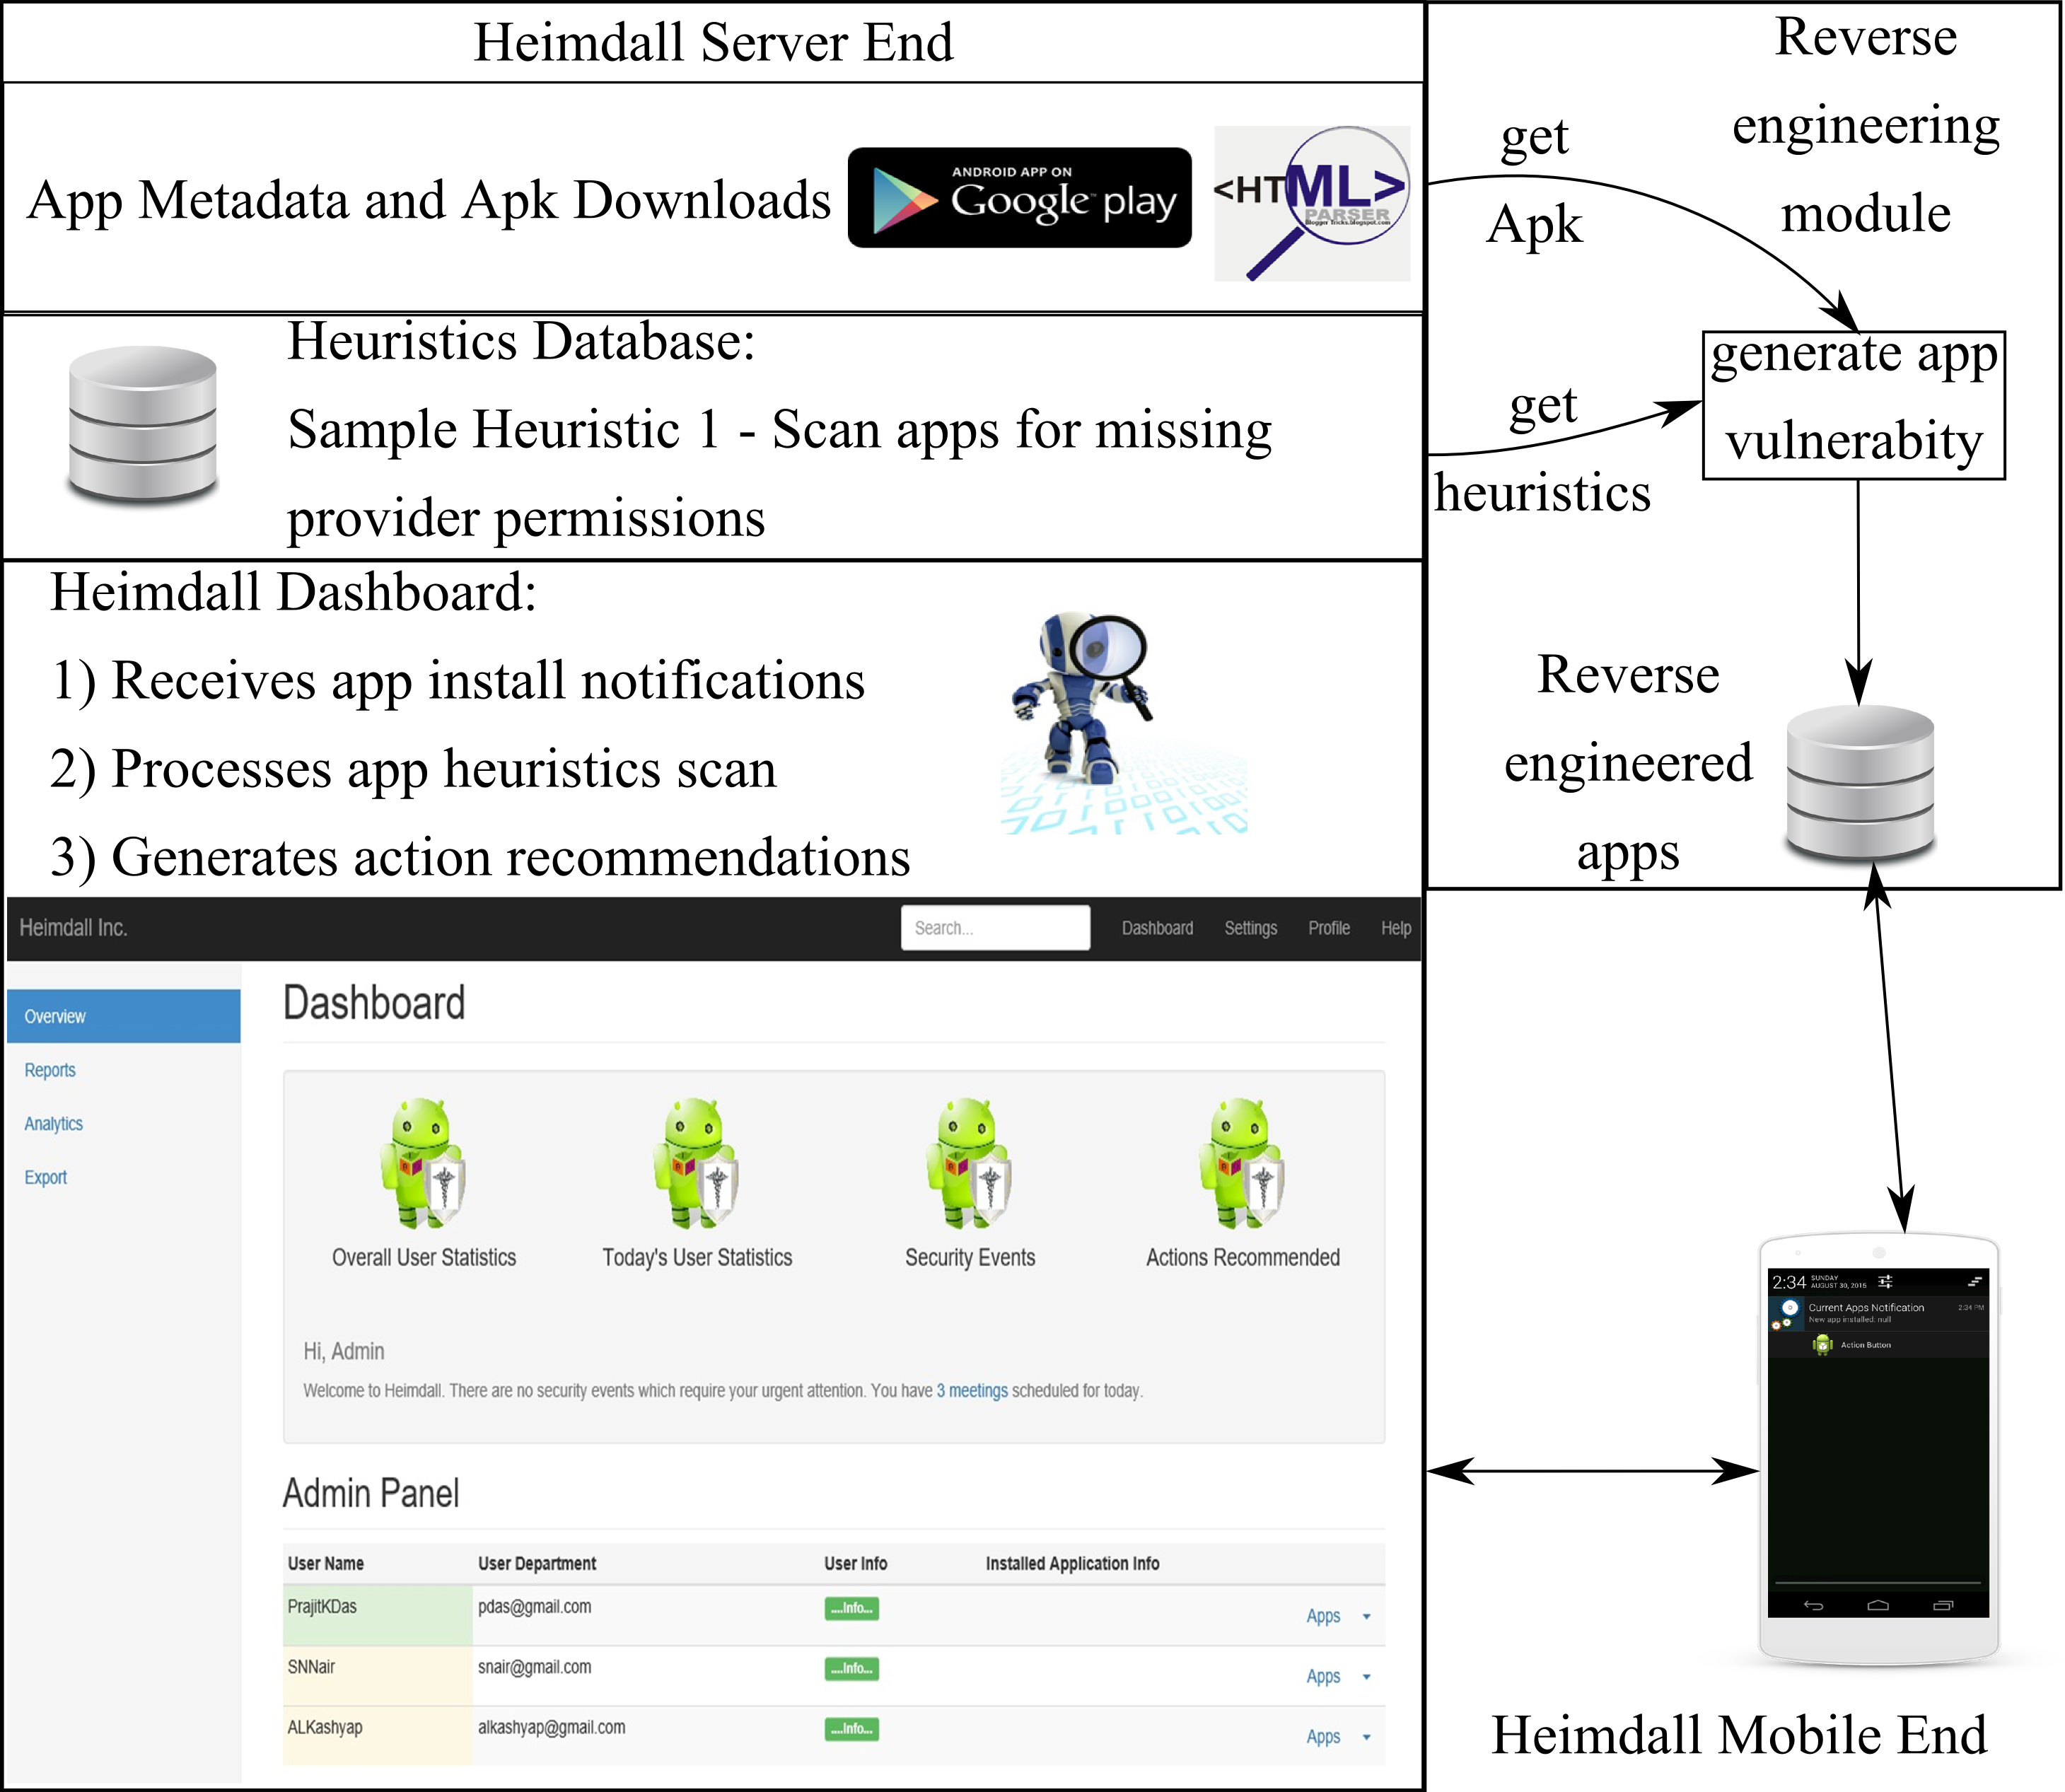
\includegraphics[width=\columnwidth]{images/architecture}
	\caption{System Overview}
	\label{fig:arch}
\end{figure}

Heimdall server has two additional capabilities. The first is to generate reverse engineered apps that we then test on the mobile devices. The reverse engineering process removes any provider associated permission and ensures that the ``exported'' tag for the provider is set to true. The second capability is to scan for missing provider permissions for known apps. For this purpose we downloaded about 1500 apps from the Google Play Store and then we use the \footnote{apktool~\url{https://ibotpeaches.github.io/Apktool/}} package to decompile the apks and parse the manifest files to determine if any of the app's provider is missing the permission association. Naturally, as we include more heuristics, Heimdall will become capable of detecting much more such vulnerability.

%\begin{figure}[tb]
	%\centering
	%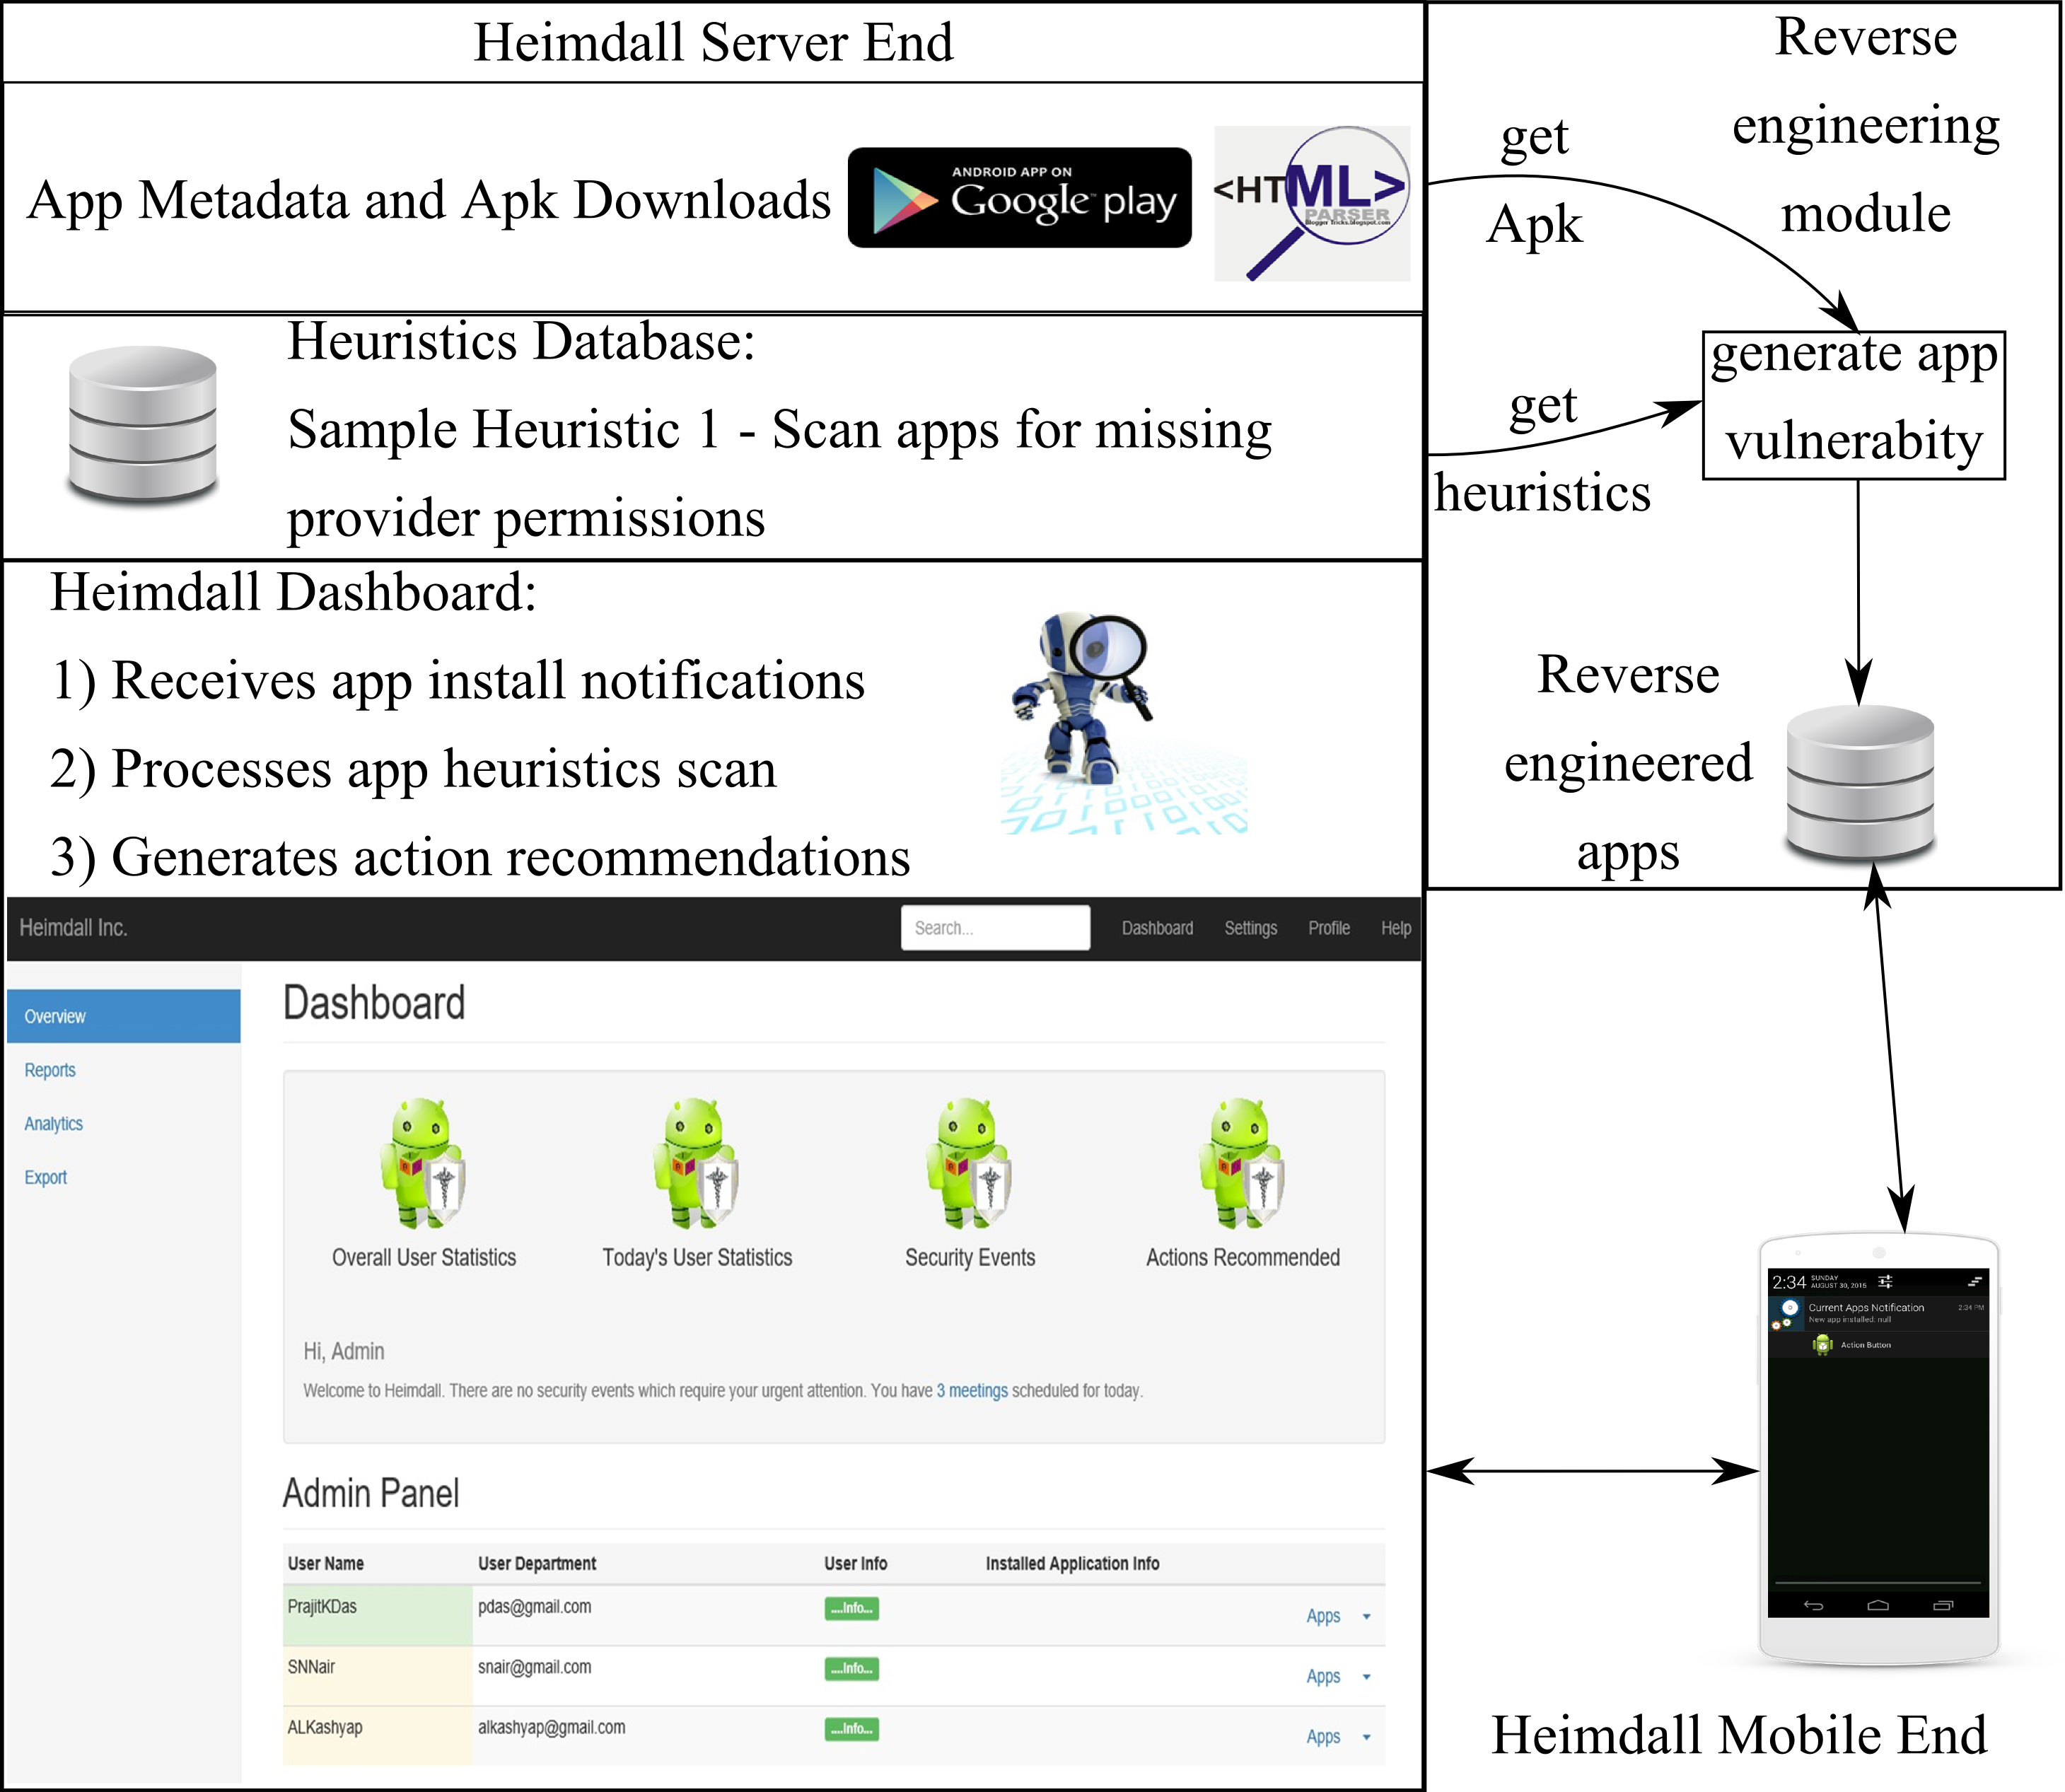
\includegraphics[width=\columnwidth]{images/architecture}
	%\caption{System Architecture}
	%\label{fig:arch}
%\end{figure}
